\documentclass[11pt,a4paper,oneside]{mythesis_mtr}

\usepackage{lscape}
\usepackage[round]{natbib}
%\usepackage{subfigure}
\usepackage{graphicx}
\usepackage{mathptm}
\usepackage{amsmath}
\usepackage{latexsym,flafter,afterpage,amssymb,color}
\usepackage{verbatim}
\usepackage{rotating}
\usepackage{setspace}
\usepackage{caption}
\usepackage{subcaption}
\doublespacing

% Use Adobe Times Roman (for printing)
%\renewcommand{\rmdefault}{ptm}
\usepackage{palatino}
%\usepackage{doublespace}

% Multicolumns in tables, shading in tables,tables to appear over multiple pages
\usepackage{multirow,colortbl,longtable}



% Page setup
\topmargin=-0.41in
\textwidth=6.5in%6.5
\textheight=9.8in
\headsep=24pt
\oddsidemargin=4mm
\parindent=0.3in
\parskip=0.1in

\newlength{\rulewidth}
\setlength{\rulewidth}{6.5in} % change to 150mm for printing on
                  % gordon, 149 otherwise???

\pagestyle{headings}

\setcounter{secnumdepth}{5}              %Numbers subsubsections, and lower.
\setcounter{tocdepth}{5}                 %Sets depth of toc to include subsubsections.



% bibliography is in a folder
%\newcommand{\BIB}{/home/swr06rsc/Documents/latex}
\newcommand{\BIB}{..}

% a bunch of useful shortcuts

\newcommand{\deriv}[2]{\frac{d #1}{d #2}}
\newcommand{\pderiv}[2]{\frac{\partial #1}{\partial #2}}
\newcommand{\tderiv}[2]{\frac{D #1}{D #2}}
\newcommand{\vect}[1]{{\bf #1}}
\newcommand{\pd}[2]{\frac{\partial^2 #1}{\partial #2^2}}

%\textwidth=149mm

\sloppy

% 1.5 line spacing so my supervisor can scrawl all over it
\renewcommand{\baselinestretch}{1.5}

% Tell latex not to mind if 0.75 of a page is full of floats
%\renewcommand{\floatpagefraction}{0.99}

% Text to put in the header

%\makeglossary

\begin{document}
  %format document

%Title page and other preface elements
\pagenumbering{roman}
%Title page

\begin{titlepage}
\begin{flushright}
\begin{figure}[h]
\begin{flushright}
  \vspace{-2cm}
\includegraphics[width=50mm]{preface/figures/reading_logo.pdf} %pdf for use with pdflatex
\end{flushright}
\end{figure}
\end{flushright}
\begin{flushleft}
  \vspace{4cm}
\Huge{\bf{Understanding the information content in diverse observations of forest carbon stocks and fluxes for data assimilation and ecological modelling}}\\ %title of PhD
\huge{PhD in Atmosphere, Oceans and Climate} \\ %PhD course
\Large{\bf{Department of Meteorology}}\\ %Department
\vspace{2cm}
\huge{Ewan Mark Pinnington} \\ %name
\Large{\bf{February 2017}}\\ %submission date
\end{flushleft}
\end{titlepage}



%Updated for UoReading regulations by Emma Dodd

\chapter{Declaration}
\vspace*{2\baselineskip}
I confirm that this is my own work and the use of all material from other sources has
been properly and fully acknowledged.
\vspace{6\baselineskip}\\
\begin{flushright}
\hspace*{\fill}
Una Person
\newline
September 2003
\end{flushright}


\cleardoublepage

\chapter*{\centering \Large \vspace{-20mm}\Huge Publications}

%=========================================================
%Abstract goes here

\nobibliography*

The work in chater~\ref{chap:error_corrs} and \ref{chap:disturbance} of this thesis has appeared in the following publications:

\bibentry{Pinnington2016299}

\bibentry{Pinnington2017}

All work undertaken in these publications was carried out by Ewan Pinnington with co-authors providing guidance and review. Matthew Wilkinson also provided data from the Alice Holt flux tower.

\chapter*{\centering \Large \vspace{-20mm}\Huge Abstract}

%=========================================================
%Abstract goes here

Forest are important here is some stuff to better understand them!

%Acknowledgements
\chapter*{\centering \Large \vspace{-20mm}\Huge Acknowledgements}

Acknowledgements go here.

\vspace{2cm}

\newpage

\tableofcontents

%Thesis start
\pagenumbering{arabic}

\chapter{Introduction}
\label{chap:intro}
%Chapter 1

\section{The global carbon cycle} \label{chap1:sec:global_c_cycle}

Carbon is one of the most abundant elements, making up around half of all living dry mass on Earth. The global carbon cycle describes the movement of carbon through the Earth system. In the Earth system large amounts of carbon are present in the oceans, atmosphere, land surface and crust. These stores of carbon are referred to as reservoirs or pools. The amount of carbon in this system can be considered constant, given that nuclear transmutation is not common under terrestrial conditions. Therefore terrestrial processes involving carbon can only transfer it between the global carbon pools. This is referred to as a flux. In pre-industrial times, the fluxes of carbon between different pools has only varied over long time scales (\(\sim\)100000 years) \citep{luthi2008high}.

The greenhouse effect describes the process by which gases (CO\(_{2}\), water vapour, ozone, etc.) in the Earth's atmosphere contribute to the warming of the planet by absorbing long-wave radiation emitted from the Earth's surface and reradiating this absorbed energy in all directions, causing more warming below \citep{mitchell1989greenhouse}. The natural greenhouse gas effect raises the global mean surface temperature by 30K, making the Earth habitable for its many lifeforms. The increase in atmospheric greenhouse gases due to anthropogenic activities since the industrial revolution, has amplified the greenhouse effect and resulted in increased global warming. CO\(_{2}\) has been found to be the most important human-contributed compound to this warming \citep{Falkowski291}. In figure~\ref{chap1:fig:ipcc_fig6.1} we show a simplified schematic of the global carbon cycle taken from the fifth Intergovernmental Panel on Climate Change (IPCC) report. In this schematic we can see the large rise in atmospheric CO\(_{2}\) since the industrial revolution up to 2011, with an increase of 240 Pg C.

\begin{figure}[ht]
    \centering
    \includegraphics[width=0.9\textwidth]{chapter/chapter1/ipcc_fig6_1.jpg}
    \caption{Global carbon cycle simplified schematic \citep{ciais2014carbon}. Black numbers and arrows represent reservoir mass and exchange fluxes estimated for the time prior to the industrial era (\(\sim\)~1750). Red numbers and arrows represent annual fluxes averaged over the 2000-2009 time period. Red numbers in the reservoirs indicate the cumulative change of carbon over the industrial period (1750-2011).}
    \label{chap1:fig:ipcc_fig6.1}
\end{figure}

As atmospheric CO\(_{2}\) levels have risen, natural sinks of CO\(_{2}\) (fluxes out of the atmosphere) have intensified with both the land surface and oceans absorbing more CO\(_{2}\) from the atmosphere than in pre-industrial times. This can be see in figure~\ref{chap1:fig:ipcc_fig6.1}, with the the net ocean flux of CO\(_{2}\) to the atmosphere decreasing from an estimated +0.7~Pg~C~yr\(^{-1}\) to -2.3~Pg~C~yr\(^{-1}\), and the land surface flux of CO\(_{2}\) to the atmosphere decreasing from -1.7~Pg~C~yr\(^{-1}\) to -2.6~Pg~C~yr\(^{-1}\). More recent estimates from \citet{le2015global} indicate these sinks have further intensified with the ocean sink estimated to be 2.9 \(\pm 0.5\)~Pg~C~yr\(^{-1}\) and the land surface sink 4.1 \(\pm 0.9\)~Pg~C~yr\(^{-1}\) for the year 2014. The intensification of the land carbon sink is thought to be partly due to a combination of forest regrowth as well as rising CO\(_{2}\) and increased nitrogen deposition having a fertilisation effect \citep{ciais2014carbon}. It has also been shown that the land surface sink has been enhanced by an increase in diffuse photosynthetically active radiation as a result of increased cloud cover associated with increased anthropogenic emissions \citep{Mercadodiffuseradiation2009}. 

The partitioning of global carbon fluxes between emissions and sinks is important to better model the carbon cycle. However, current estimates are subject to high levels of uncertainty, which are reflected by the errors shown in Figure~\ref{chap1:fig:ipcc_fig6.1}. Current best estimates of global CO\(_{2}\) emissions and their partitioning between atmospheric growth rate and sinks are shown in Figure~\ref{chap1:fig:ipcc_fig6.8}. It is vitally important to understand the future response of sinks of CO\(_{2}\) (land surface and oceans) to climate change. If either the oceans or land surface were to stop absorbing the same percentage of CO\(_{2}\), we would see even more dramatic increases in atmospheric CO\(_{2}\) levels and thus a much greater rate of global warming. There is a high level of confidence that ocean carbon uptake will continue under all future emission scenarios \citep{ciais2014carbon}. There is much less confidence for the land surface and \citet{1748-9326-7-2-024002} have shown that global warming is particularly sensitive to land surface carbon cycle processes, highlighting the need to improve understanding of land surface carbon uptake. Some estimates show the land surface changing from a sink of CO\(_{2}\) to a source of CO\(_{2}\) under certain future emission scenarios \citep{sitch2008evaluation, cox2000, scholze2006climate}. In the latest IPCC report land surface carbon uptake is still considered the least understood process in the global carbon cycle \citep{ciais2014carbon}.

\begin{figure}[ht]
    \centering
    \includegraphics[width=0.9\textwidth]{chapter/chapter1/ipcc_fig6_8.jpg}
    \caption{Annual anthropogenic CO\(_{2}\) emissions and their partitioning among the atmosphere, land and ocean from 1750 to 2011  \citep{ciais2014carbon}.}
    \label{chap1:fig:ipcc_fig6.8}
\end{figure}

Currently land surface carbon uptake is estimated by taking the residual of all other calculated sources and sinks of carbon, so that
\begin{equation}
S_{LAND} = E_{FF} + E_{LUC} - (G_{ATM} + S_{OCEAN})
\end{equation}  
where \(S_{LAND}\) is the global residual land sink of CO\(_{2}\), \(E_{FF}\) is the CO\(_{2}\) emissions from fossil fuels, \(E_{LUC}\) is the CO\(_{2}\) emissions from land use change (mainly deforestation), \(G_{ATM}\) is the atmospheric CO\(_{2}\) growth rate and \(S_{OCEAN}\) is the mean ocean CO\(_{2}\) sink \citep{le2015global}. Figure~\ref{chap1:fig:ipcc_fig6.8} shows the growth in the estimated residual land sink as emissions increase. The high variability shown in this sink is largely due to the fact that it contains the residual errors of the four other terms. However, the land sink also displays some variability due to its sensitivity to year to year variations in precipitation, surface temperature, radiation and volcanic eruptions. Figure~\ref{chap1:fig:ipcc_fig6.8} shows that in 1986 and 1997 the land sink drops to zero, both of these years were among the strongest El Ni\~no's in recent history. In 1997 tropical droughts, often associated with El Ni\~no, were particularly severe leading to wildfires that released vast amounts of stored carbon \citep{schimel2013climate}.

%{\color{red} Include ecosystem flux description and figure here}
Terrestrial ecosystems are made up of autotrophs (organisms capable of photosynthesis) and heterotrophs (organisms that feed on organic carbon). The Gross Primary Productivity (GPP) of an ecosystem is the total amount of carbon removed from the atmosphere by photosynthesis. The Total Ecosystem Respiration (TER) is made up of autotrophic respiration (e.g. from plants) and heterotrophic respiration (e.g. from soil and litter organisms). The total carbon uptake or Net Ecosystem Exchange (NEE) of CO\(_2\) is then equal to -GPP+RT. A representation of these fluxes for a forest ecosystem are shown in Figure~\ref{chap1:fig:eco_fluxes}. 

\begin{figure}[ht]
    \centering
    \includegraphics[width=0.5\textwidth]{chapter/chapter1/flux.pdf}
    \caption{Fluxes of carbon through a forest ecosystem. Gross Primary Productivity (GPP) represents total photosynthesis, R\(_{\text{a}}\) is autotrophic respiration from foliage, wood and roots, R\(_{\text{h}}\) is heterotrophic respiration from soil and litter. Total ecosystem respiration of carbon to the atmosphere (RT) is equal to R\(_{\text{a}}\) + R\(_{\text{h}}\). The Net Ecosystem Exchange (NEE) of CO\(_{2}\) is equal to -GPP + RT.}
    \label{chap1:fig:eco_fluxes}
\end{figure}

Disturbance of terrestrial ecosystems from fire, felling and insect outbreak can have significant impacts on carbon dynamics. Land use change is the second largest anthropogenic source of CO\(_{2}\). However, It is not well understood how much CO\(_{2}\) is removed from the atmosphere by regrowth of previously disturbed ecosystems (either by felling or fire), although it is thought that regrowth of forests in partcular could be stronger carbon sinks than their predecessors, due to more rapid biomass accumulation under succession \citep{pan2011large}. Better understanding the response of the land surface to disturbance will help constrain future carbon budgets. 

%Good paper to highlight the fact that the percentage of CO\(_{2}\) absorbed by the land surface has remained approximately constant with rising atmospheric CO\(_{2}\) levels??? Maybe just use IPCC fig 6.8?

%In figure 6.1 and 6.8: Partitioning of fluxes important and hard (shown by error on estimates in fig 6.1). Land surface carbon uptake least understood mechanism in the global carbon cycle, ref IPCC. Will uptake remain the same under climate change.

%Human emissions of CO\(_{2}\) have perturbed the global C cycle and caused a large continual increase in atmospheric CO\(_{2}\) levels.

%Look at papers recommended on Flux Course, some good ones to reference???

%IPCC figure 6.1 and 6.8: Partitioning of fluxes important and hard (shown by error on estimates in fig 6.1). Land surface carbon uptake least understood mechanism in the global carbon cycle, ref IPCC. Will uptake remain the same under climate change.

%\citet{1748-9326-7-2-024002} Have shown that global warming is highly sensitive to land carbon cycle processes and highlighted the need to improve understanding of land surface carbon uptake and its response to climate change. 

\section{Observations of terrestrial carbon balance}

There are an increasing number of available observations relevant to understanding the carbon balance of forests and the terrestrial biosphere. These observations include a range of variables, perhaps two of the most common are the Net Ecosystem Exchange (NEE) of CO\(_{2}\) and Leaf Area Index (LAI), which is the area of leaves per unit area ground. These variables can be directly measured at site level and can also be estimated from satellite remote sensing. Both NEE and LAI are important variables for understanding the carbon balance of ecosystems, with NEE giving us a direct estimate of the carbon uptake of an ecosystem and LAI being a main driver for the amount of GPP an ecosystem can perform.

%para on flux network and site level data:
At site level, flux towers measuring ecosystem-atmosphere fluxes of CO\(_{2}\), water and energy using the micrometeorological technique of eddy covariance provide one of the most valuable sources of information. Direct observations of ecosystem CO\(_{2}\) uptake are made at a fine temporal resolution, with observations every half-hour. A global flux network (FLUXNET), was established in 1997 \citep{baldocchi2001fluxnet}, to consolidate the information from a growing number of flux tower sites. Currently there are 517 active FLUXNET sites which are shown in Figure~\ref{chap1:fig:fluxnet_2015}, as can be seen these sites are not uniformly distributed so it is not possible to use FLUXNET sites alone to produce global estimates of terrestrial CO\(_{2}\) balance. However, these sites do provide an invaluable resource for model and satellite calibration. In turn this can be used to produce estimates on a global scale. At many flux tower sites and forest stands other diverse observations relevant to terrestrial carbon budgets are also being made. These include observations of soil and litter respiration, woody biomass and LAI. However, because they are labour intensive these observations are made much less frequently.     

\begin{figure}[ht]
\centering
\includegraphics[width=0.9\textwidth]{chapter/chapter1/FluxNetworkMODIS_IGBP_10-2015.png}
\caption{FLUXNET sites and land cover (MODIS IGBP classification) \citep{fluxnetsite2013}.}
\label{chap1:fig:fluxnet_2015}
\end{figure}

%para on satellite data
The Moderate Resolution Imaging Spectroradiometer (MODIS) on the TERRA and AQUA satellites produces global estimates of LAI and Gross Primary Productivity (GPP) for terrestrial ecosystems \citep{running2004continuous}. However, MODIS actually measures reflected sunlight, this is then converted to vegetation indices, such as the Normalised Difference Vegetation Index (NDVI). These indices are correlated with the fraction of absorbed visible sunlight to estimate LAI or used in simple algorithms to estimate GPP \citep{yuan2007deriving}. It is therefore important to understand the limitations when interpreting satellite products as they do not represent direct observations. For LAI it has been shown that remotely sensed estimates saturate when measuring ecosystems with a LAI above 3 \citep{myneni2002global}. Terrestrial fluxes of carbon estimated from satellite measurements are subject to large errors in representativity, as satellites view a scene almost instantaneously and then derive daily mean fluxes \citep{baldocchi2008turner}. 
%Baldocchi paper: Many observations of forest carbon flux made worldwide.

\section{The role of models}

Observations can only tell us about the current and past state of a system. In order to produce future predictions and better understand current terrestrial carbon dynamics we must use mathematical models. Figure~\ref{chap1:fig:ipcc_fig6.16} show a comparison of the residual land sink (described in section~\ref{chap1:sec:global_c_cycle}) with the global terrestrial CO\(_{2}\) sink estimated from different process based global carbon cycle models. We see that although there is a high variability between modelled estimates there is good agreement between the multi-model mean and the residual land sink. 

\begin{figure}[ht]
    \centering
    \includegraphics[width=0.9\textwidth]{chapter/chapter1/ipcc_fig6_16.jpg}
    \caption{Comparison of the residual land sink (black line) with the global terrestrial CO\(_{2}\) sink estimated from different process based global carbon cycle models \citep{ciais2014carbon}. Grey shading represents uncertainty in residual land sink.}
    \label{chap1:fig:ipcc_fig6.16}
\end{figure}

Representative Concentration Pathways (RCPs) of CO\(_{2}\) concentrations and emissions have been developed \citep{moss2010next} to drive climate models to produce future predictions. Under these pathways land surface carbon uptake is highly uncertain with little agreement between different process based models. Some predict the land surface to become a source of CO\(_{2}\) and others predict a further intensification of the residual land sink \citep{jones2013twenty}. This large uncertainty for land surface models is partly due to poor model parameterisations and missing processes within models. One of the main processes many current global models do not account for is the effect of disturbance on terrestrial ecosystem carbon dynamics.

It has been shown that many terrestrial carbon cycle models simulating the seasonal cycle of land-atmosphere CO\(_{2}\) exchange perform poorly when compared to FLUXNET sites in North America \citep{schwalm2010model}. Here a difference between observations and model predictions of 10 times the observational uncertainty was found, highlighting the need for continued model development. In order to improve global models of terrestrial carbon balance it is important to use site-level-research to hone the processes and parameterisations of the models where we have diverse sets of direct observations with which to judge modified-model performance. 
%IPCC figure 6.16 and section 6.3.2.6.6: Contribution of models to understanding the terrestrial carbon cycle. Reference every DALEC paper.


\section{Data assimilation}

%{\color{red} Observations are sparse, current model predictions are poor, data assimilation provides a way to combine both sources of information to improve current estimates.}

As discussed above, the level of uncertainty in terrestrial carbon balance predictions arise from significant gaps in the direct observations available and from a lack of clarity and authoritative parameterisation of the constituent processes in current models. The technique of data assimilation provides a method for combining and comparing the output of predictive models with incomplete observations to find the best estimate for the state and parameters of a system. Data assimilation has had many successful applications. Perhaps the most important application has been in numerical weather prediction where data assimilation has contributed to forecast accuracy being increased at longer lead times, with the result that the four day forecast in 2014 now has the same level of accuracy as the one day forecast in 1979 \citep{bauer2015quiet}. Obviously, this improved forecasting is not solely due to data assimilation but also increased quality and resolution of observations along with improvements in model structure, however the introduction and evolution of data assimilation has been a key part of the improvement \citep{dee2011era}.

More recently data assimilation has been used to improve our knowledge of ecological systems. For the carbon balance of forests it has been used to combine many different observations with functional ecology models \citep{zobitz2011primer, fox2009reflex, richardson2010estimating, Quaife2008, Zobitz2014, Niu2014}. Global land surface models have also been implemented with data assimilation, mainly using data from satellite and atmospheric $\text{CO}_{2}$ observations \citep{Kaminski2013, scholze2007propagating}. In a few cases site level data has also been assimilated \citep{Verbeeck2011, Bacour2015}. In comparison with numerical weather prediction, the use of data assimilation in these areas is relatively new and underdeveloped. The further application of data assimilation to models of ecosystem carbon balance will help to improve model parameterisations and future predictions. The development of improved data assimilation techniques will also help to  identify missing model processes and changes in model parameters and behaviour over time. In particular, understanding the change in model parameters over time will be of use in improving models predictions of the effect of disturbance in terrestrial ecosystems.
  
%Role of DA in NWP improving forecast skill. 



%\chapter{Thesis aims and outline}
%\label{chap:aims}
%Chapter 2: Thesis aims and outline

We aims to do this and that

\begin{itemize}
\item UNderstanding this!
\item investigating that!
\item Using something else!
\end{itemize}

%Figure Example:

%\begin{figure}[htbp]
%\centering
%\includegraphics[trim=5pc 20pc 5pc 20pc, clip=true, width=0.8\textwidth]{chapter/chapter2/ch2fig1}
%\caption{\small Annual anomalies of global land-surface air temperature ($^\circ$C), 1850 to 2005 from several datasets. The smooth curves show decadal variations. Figure 3.1 from Climate Change 2007: The Physical Science Basis. Contribution of Working Group I to the Fourth Assessment Report of the Intergovernmental Panel on Climate Change.}
%\label{ch2fig1}
%\end{figure}


\chapter{Current state of data assimilation for the carbon cycle}
\label{chap:litrev}
%Chapter 3


\section{Data assimilation methods}

Data assimilation provides techniques for combining observations and prior knowledge of a system in an optimal way to find an improved estimate of the system. The prior knowledge of a system often takes the form of a numerical model and an initial guess of the model state/parameters. Many statistical methods have been developed for data assimilation. These methods can largely be categorised as either sequential or variational. Sequential algorithms solve the system of equations needed to find an optimal solution explicitly at each observation time. Variational methods solve the equations needed for an optimal solution implicitly by minimising a cost function for all available observations over some time window. This thesis is mainly concerned with the variational technique of four-dimensional variational data assimilation (4D-Var). 

In numerical weather prediction data assimilation has been predominately used for state estimation whilst keeping parameters fixed. This is because numerical weather prediction is mainly dependent on the initial state with model physics being well understood. Ecosystem carbon cycle models are more dependent on finding the correct set of parameters to describe the ecosystem of interest \citep{luo2015predictability}. We therefore discuss data assimilation for joint state and parameter estimation. In the next sections (\ref{chap3:sec:intro_da} to \ref{chap3:sec:mcmc_seq}) we give a general introduction to data assimilation, then expand this to 4D-Var and finally we briefly discuss other data assimilation methods not directly used in this thesis but applicable to subsequent discussion. 

\subsection{Introduction to data assimilation} \label{chap3:sec:intro_da}

We consider a system that can be described by a numerical model with a true model state \(\textbf{z}^{t} \in \mathbb{R}^{n}\) and true parameters \(\textbf{p}^{t} \in \mathbb{R}^{q}\). We then define the true augmented state as
\begin{equation}
\textbf{x}^{t} =
\begin{pmatrix}
\textbf{p}^{t} \\
\textbf{z}^{t}
\end{pmatrix}
\in \mathbb{R}^{q+n}.
\end{equation}
The initial guess to this model augmented state \(\textbf{x}^{b} \in \mathbb{R}^{q+n}\) (often referred to as the prior or background) and observations of the system \(\textbf{y} \in \mathbb{R}^{m}\) will only be approximations to the true system state, such that
\begin{equation}
\textbf{x}^{b} = \textbf{x}^{t} + \bm{\epsilon}^{b}, \label{chap3:eqn:xb}
\end{equation} 
\begin{equation}
\textbf{y} = h(\textbf{x}^{t}) + \bm{\epsilon}^{o}, \label{chap3:eqn:y}
\end{equation} 
where \( \bm{\epsilon}^{b}\) and \( \bm{\epsilon}^{o}\) are the prior and observation errors respectively, and \(h: \mathbb{R}^{q+n}\rightarrow \mathbb{R}^{m}\) is the observation operator (can be linear or non-linear) mapping the augmented state to observation space, for example the nonlinear mapping of carbon pool state and parameters to eddy covariance derived observations of NEE. The errors in the prior and observations are assumed to be unbiased and mutually independent with known covariance matrices \(\textbf{B} = \mathbb{E}[\bm{\epsilon}^{b}(\bm{\epsilon}^{b})^{T}]\) and \(\textbf{R} = \mathbb{E}[\bm{\epsilon}^{o}(\bm{\epsilon}^{o})^{T}]\).

The best estimate to \(\textbf{x}^{t}\) satisfying both equation~\eqref{chap3:eqn:xb} and \eqref{chap3:eqn:y} is often called the analysis or the posterior estimate, here denoted \(\textbf{x}^{a}\). It is possible to derive this analysis by applying Bayesian methods to probability density functions. Bayes' theorem is first discussed in \citet{bayes1763} but formalised by \citet{laplace1781memoire}. Applied to probability density functions (pdf's) Bayes theorem can be expressed mathematically as
\begin{equation}
p^a(\textbf{x}|\textbf{y}) \propto p^b(\textbf{x})p^o(\textbf{y}|\textbf{x}), \label{chap3:eqn:bayes}
\end{equation}
where \(p^b(\textbf{x})\) is the pdf for the prior, \(p^o(\textbf{y}|\textbf{x})\) is the pdf of the observations given the augmented state and \(p^a(\textbf{x}|\textbf{y})\) is the posterior pdf for the augmented state. Maximising the probability \(p^a(\textbf{x}|\textbf{y})\) is then equivalent to finding the augmented state that best represents the observations. 

If we make the assumption of Gaussian probability density functions with
\begin{equation}
p^{b}(\textbf{x}) = \frac{1}{\sqrt{2\pi |\textbf{B}|^{(q+n)}}}\text{exp}\big(-\frac{1}{2}(\textbf{x}-\textbf{x}^{b})^{T}\textbf{B}^{-1}(\textbf{x}-\textbf{x}^{b})\big)
\end{equation}
and
\begin{equation}
p^{o}(\textbf{y}|\textbf{x}) = \frac{1}{\sqrt{2\pi |\textbf{R}|^{m}}}\text{exp}\big(-\frac{1}{2}(\textbf{y}-h(\textbf{x}))^{T}\textbf{R}^{-1}(\textbf{y}-h(\textbf{x}))\big).
\end{equation}
Then from Bayes' theorem (equation~\eqref{chap3:eqn:bayes}) the posterior probability density function for the augmented state
\begin{equation}
p^{a}(\textbf{x}|\textbf{y}) \propto \text{exp}\big(-\frac{1}{2}(\textbf{x}-\textbf{x}^{b})^{T}\textbf{B}^{-1}(\textbf{x}-\textbf{x}^{b})-\frac{1}{2}(\textbf{y}-h(\textbf{x}))^{T}\textbf{R}^{-1}(\textbf{y}-h(\textbf{x}))\big), \label{chap3:eqn:p_x_y}
\end{equation} 
here we can ignore the constant multiplying the exponential function as it is independent of \textbf{x}. We want to maximise the probability of the augmented state \textbf{x} given the observations \textbf{y}. From equation~\eqref{chap3:eqn:p_x_y} we can see that to maximise \(p^{a}(\textbf{x}|\textbf{y})\) we must maximise the terms in the exponent, this is equivalent to minimising the quadratic cost function 
\begin{equation}
J(\textbf{x}) = \frac{1}{2}(\textbf{x}-\textbf{x}^{b})^{T}\textbf{B}^{-1}(\textbf{x}-\textbf{x}^{b}) + \frac{1}{2}(\textbf{y}-h(\textbf{x}))^{T}\textbf{R}^{-1}(\textbf{y}-h(\textbf{x})). \label{chap3:eqn:3dvar}
\end{equation}
This is the cost function minimised in three-dimensional variational data assimilation (3D-Var), where the minimum is found using a descent algorithm evaluating equation~\eqref{chap3:eqn:3dvar} and its gradient \citep{courtier1998ecmwf}. We can approximate the minimum of \eqref{chap3:eqn:3dvar} by finding its gradient and setting it to zero to obtain the Best Linear Unbiased Estimate (BLUE) \citep{talagrand1997assimilation} where
\begin{equation}
\textbf{x}^{a} = \textbf{x}^{b} + \textbf{K}(\textbf{y} - h(\textbf{x}^{b})), \label{chap3:eqn:blue}
\end{equation}
\begin{equation}
\textbf{K} = \textbf{B}\textbf{H}^{T}(\textbf{H}\textbf{B}\textbf{H}^{T}+\textbf{R})^{-1},
\end{equation}
where \textbf{K} is the Kalman gain matrix specifying the weight of the analysis increment and \(\textbf{H}=\frac{\partial h(\textbf{x})}{\partial \textbf{x}}\) is the linearised observation operator (linearised around \(\textbf{x}=\textbf{x}^{b}\)). We can also approximate the analysis error covariance matrix as
\begin{equation}
\textbf{A} = (\textbf{H}^{T}\textbf{R}^{-1}\textbf{H}+\textbf{B}^{-1})^{-1}. \label{chap3:eqn:a_cov}
\end{equation}
If \( h \) is linear then \eqref{chap3:eqn:blue} and \eqref{chap3:eqn:a_cov} are exact solutions.
%(BLUE) introduce basic concept of DA for a linear Gaussian time-invariant system... will use this in Info Con chapter

%BLUE \(\rightarrow\) 3D-Var

\subsection{4D-Var} \label{chap3:sec:4dvar}

%*Brief* but inclusive of all notation need for results chapter on information content
Four dimensional variational data assimilation (4D-Var) extends 3D-Var to allow for the assimilation of observations distributed throughout some time interval \(t_{0}\) to \(t_{N}\). \citet{Sasaki70somebasic} proposed a method for combining a time series of observations with a numerical model, which was then further developed for use in numerical weather prediction \citep{dimet1986variational}. In 4D-Var we minimise the cost function,
\begin{equation}
\begin{split}
J(\textbf{x}_0) &= J_b(\textbf{x}_0) + J_o(\textbf{x}_0) \\
&= \frac{1}{2}(\textbf{x}_0-\textbf{x}^b)^{T}\textbf{B}^{-1}(\textbf{x}_0-\textbf{x}^b)+\frac{1}{2}\sum_{i=0}^{N}(\textbf{y}_i-\textbf{h}_i(\textbf{x}_i))^{T}\textbf{R}_{i,i}^{-1}(\textbf{y}_i-\textbf{h}_i(\textbf{x}_i)), \label{chap3:eqn:4dvar_cost}
\end{split}
\end{equation}
to obtain the analysis \(\textbf{x}^{a}_{0}\), valid at the initial time \(t_{0}\), subject to the strong constraint that the model states (\(\textbf{x}_0, \dots, \textbf{x}_N\)) must satisfy the model equations,
\begin{equation}
\textbf{x}_{i} = \textbf{m}_{i-1 \rightarrow i}(\textbf{x}_{i-1}), \label{chap3:eqn:nonlinmod}
\end{equation}
where \(\textbf{x}_{i}\) is the model augmented state at time \(t_i\), \(\textbf{m}_{i-1 \rightarrow i}\) is the possibly nonlinear augmented system model evolving \(\textbf{x}_{i-1}\) from time \(t_{i-1}\) to time \(t_i\), \(\textbf{y}_i\) is the vector of observations at time \(t_i\), \(h_i\) is the observation operator at time \(t_i\), and \(\textbf{R}_{i,i}\) is the observation error covariance matrix at time \(t_i\). The time evolution model for the parameter components of the augmented system is just \(\textbf{p}_i = \textbf{p}_{i-1}\), so that the model parameters are constant in time. We can generalise equation~\eqref{chap3:eqn:4dvar_cost} to avoid the sum notation as
\begin{equation}
J(\textbf{x}_0) = \frac{1}{2}(\textbf{x}_0-\textbf{x}^b)^{T}\textbf{B}^{-1}(\textbf{x}_0-\textbf{x}^b)+\frac{1}{2}(\hat{\textbf{y}}-\hat{\textbf{h}}(\textbf{x}_0))^{T}\hat{\textbf{R}}^{-1}(\hat{\textbf{y}}-\hat{\textbf{h}}(\textbf{x}_0)), \label{chap3:costfn}
\end{equation}
where,
\begin{equation}
\hat{\textbf{y}} =
\begin{pmatrix}
\textbf{y}_0 \\
\textbf{y}_1\\
\vdots \\
\textbf{y}_N
\end{pmatrix},
\hspace{1mm}
\hat{\textbf{h}}(\textbf{x}_0)=
\begin{pmatrix}
\textbf{h}_0(\textbf{x}_0) \\
\textbf{h}_1(\textbf{m}_{0\rightarrow 1}(\mathbf{x}_{0}))\\
\vdots \\
\textbf{h}_N(\textbf{m}_{0\rightarrow N}(\mathbf{x}_{0}))
\end{pmatrix}, \\
\hspace{1mm} \text{and} \hspace{3mm}
\hat{\mathbf{R}} =
\begin{pmatrix}
\mathbf{R}_{0, 0} & \mathbf{R}_{0, 1} & \dots & \mathbf{R}_{0, N} \\
\mathbf{R}_{1, 0} & \mathbf{R}_{1, 1} & \dots & \mathbf{R}_{1, N} \\
\vdots & \vdots & \ddots & \vdots \\
\mathbf{R}_{N, 0} & \mathbf{R}_{N, 1} & \dots & \mathbf{R}_{N, N}
\end{pmatrix},
\end{equation}
with the off-diagonal blocks of \(\hat{\mathbf{R}}\) corresponding to correlations in time between observation errors. For 4D-Var we approximate the analysis error covariance matrix as
\begin{equation}
\textbf{A} = (\hat{\textbf{H}}^{T}\hat{\textbf{R}}^{-1}\hat{\textbf{H}}+\textbf{B}^{-1})^{-1}, \label{chap3:eqn:a_cov_4dvar}
\end{equation}
where \(\hat{\textbf{H}}\) is the observability matrix given by
\begin{equation}
\hat{\mathbf{H}}=
\begin{pmatrix}
\mathbf{H}_0 \\
\mathbf{H}_1\mathbf{M}_0\\
\vdots \\
\mathbf{H}_N\mathbf{M}_{N,0}
\end{pmatrix}
\end{equation}
with $\textbf{H}_i = \frac{\partial \textbf{h}_i(\textbf{x}_i)}{\partial\textbf{x}_i}$ the linearised observation operator and $\mathbf{M}_{i,0}=\mathbf{M}_{i-1}\mathbf{M}_{i-2}\cdots\mathbf{M}_0$ the tangent linear model with $\mathbf{M}_i=\frac{\partial \textbf{m}_{i-1\rightarrow i}(\textbf{x}_{i})}{\partial \textbf{x}_{i}}$. The tangent linear model can be difficult to implement, however using techniques such as automatic differentiation \citep{renaud1997automatic} can reduce the time taken to implement the derivative of a model. These techniques are employed in this thesis.

\subsection{Markov chain Monte Carlo and sequential approaches} \label{chap3:sec:mcmc_seq}

Markov chain Monte Carlo (MCMC) methods refer to a suite of related algorithms (Metropolis-Hastings, simulated annealing and Gibbs sampling), with one of the first MCMC methods being the Metropolis algorithm \citep{metropolis1953equation}. These methods sample the posterior pdf by calculating a cost function measuring the model-data mismatch at different points, usually similar to \(-J_o(\textbf{x}_0)\) shown in equation~\eqref{chap3:eqn:4dvar_cost}. As these methods use \(-J_o(\textbf{x}_0)\) they seek to find a global optimum for this cost function, rather than a minimum. This is achieved by iteratively sampling the cost function, with each iteration of the parameter and state values being uniquely determined by the previously sampled parameter and state values. The output of the MCMC methods is a set of accepted parameter and state values from which analysis or posterior error covariances can be calculated. These methods are easy to implement and do not require the derivative of the model code. However, they come with high computational cost as they often require in the order of \(10^{6}\) model evaluations even for a simple model of forest carbon balance \citep{zobitz2011primer, ziehn2012}. These methods become infeasible for global implementations of more complex models. 

Whereas variational and MCMC techniques assimilate all available observations over some time window at once, sequential algorithms update the model trajectory at each observation time. These algorithms approximate the BLUE formula in equation~\eqref{chap3:eqn:blue} to update the model parameter and state values whenever an observation is available. This means that parameter values can change over time and state and parameter analysis trajectories will become discontinuous (unless using a sequential `smoother' method). The first sequential method for linear systems was the Kalman Filter (KF) \citep{kalman1960}. The KF method requires the evolution of the error covariance matrix \textbf{B} through the time window as observations are assimilated. This becomes infeasible for large systems. The Ensemble Kalman Filter (EnKF) \citep{Evensen2003} was developed to address this problem and allow for the optimisation of nonlinear systems. Here the error covariance matrix for the state/parameters is approximated using an ensemble of state/parameter vectors. Therefore the evolution of the error covariance matrix \textbf{B} is avoided. These methods are also easy to implement. However, dependent on the complexity of the model, the ensemble size can be limited by computational cost, meaning that covariances can be subject to sampling errors. Ad hoc techniques (localisation and inflation) have been employed to reduce these problems \citep{Hamill2001, andersonandanderson1999}.

\section{Applications to the carbon cycle}

For numerical weather prediction DA is used predominantly for state estimation. However this is not true for land surface carbon balance models where parameters are much less well understood. Indeed these parameters can change over time within a developing ecosystem or when an ecosystem is subject to a disturbance event. Therefore, the vast majority of current studies use DA to estimate both parameter and state variables.

The use of DA for the estimation of parameter and state variables of ecosystem carbon models has either been at site-level, with flux tower observations and other ancillary data relevant to ecosystem carbon balance, or for global implementations, where often the implied effect of the land surface on atmospheric CO\(_{2}\) observations has been considered. It is important that we improve DA techniques both at site-level and for global implementations.   

\subsection{Site-level applications}

%Chronological order?

%Many MCMC routines, at the global scale these will become increasing difficult to implement due to computational expense
\subsubsection{Early efforts}

Two of the first examples of combining site-level eddy covariance data with models of ecosystem carbon balance were using the Data Assimilation Linked Ecosystem Carbon (DALEC) and SImplified PhotosyNthesis and EvapoTranspiration (SIPNET) models by \citet{williams2005improved} and \citet{braswell2005estimating} respectively. These are both simple process based models of ecosystem carbon dynamics. In \citet{braswell2005estimating} MCMC techniques (based on the Metropolis algorithm) are used to combine half-daily observations of NEE with the SIPNET model. The DA technique is used to estimate initial model parameter and state values as well as the standard deviation in NEE flux observation (found to be approximately \(1~\text{g C m}^{-2}\)). It is shown that NEE has limited ability to constrain some model parameters as the model prediction of NEE is insensitive to these parameters at the time-scales shown in the study (10 years). \citet{williams2005improved} assimilated a more diverse set of daily carbon flux and stock observations from the Metolius ponderosa pine site (Oregon, USA) with the DALEC model. In this study, an EnKF is nested within a quasi-Newton optimisation scheme to find the initial set of parameter and state values that require least correction by the EnKF. The use of variational or MCMC techniques is more common to estimate the initial state and parameter values of a model. \citet{williams2005improved} found large reductions in model prediction error after assimilation. They noted that rare measurements of carbon stocks had limited impact on assimilation results but suggested that longer time-series of these stock measurements will be important to constrain carbon pool turnover rates. They also assimilated modelled GPP from the more complex soil-plant-atmosphere (SPA) model \citep{williams1997predicting} and claimed that this was analogous to satellite derived GPP, as this more complex model was already calibrated for the Metolius forest. They suggested that, based on their results assimilating SPA modelled GPP, in future studies using satellite GPP products would be beneficial.  

\subsubsection{Data assimilation comparison projects} 

As data assimilation became more widespread with models and observations of ecosystem carbon dynamics \citet{trudinger2007optic} conducted the Optimisation InterComparison (OptIC) project to better understand the benefits and issues of different DA implementations. In this study participant researchers used a variety of distinct DA implementations to estimate the parameters of a highly simplified model of terrestrial carbon balance. No single DA method was found to perform better than others and the representation of the cost function was shown to be more important than the method. In different optimisation experiments the representation of error added to pseudo observations was varied (Gaussian, lognormal, temporally correlated distributions, etc.). It was stated that the main criterion for success was accurate specification of errors. In particular, none of the participant researchers made an effort to account for temporally correlated error, which resulted in biased results. \citet{williams2009improving} comment that temporal error correlations between flux measurements on the scale of a day and less are likely to be severe. They suggested that these could be included in the observation error covariance matrix, although they comment that this would be a difficult task. In section~\ref{chap6:sec:corR} we show how these correlations can be included.  

The REgional Flux Estimation eXperiment (REFLEX) was a similar study conducted by \citet{fox2009reflex} using the DALEC model. In this study, 9 participants were asked to combine both synthetic and observed NEE and LAI data with the DALEC model. Again a variety of DA methods were used (although no variational methods). No DA technique performed consistently better than others. Across all methods, the parameters linked directly to GPP and TER were best constrained, while those linked to slower processes (allocation and turnover of fine root and wood carbon pools) were poorly constrained. \citet{fox2009reflex} suggest that observations of slow large carbon pools would add useful constraint to DA schemes and compliment eddy covariance data. It is also discussed that future studies should investigate the importance of prior error estimates (we explore this in Chapter~\ref{chap:error_corrs}). The representation of prior and observational errors are still very basic in the majority of current DA schemes for ecosystem carbon balance. \citet{Dietze2013} also stress the need to improve the representation of uncertainty in DA schemes. 

As data assimilation with ecological applications becomes more prevalent it is important that tools for information management and data assimilation are made more accessible. The Predictive Ecosystem Analyser (PEcAn) is an effort to achieve this. PEcAn also allows for easier comparison of different implemented models \citep{Dietze2013} with the aim of improving the standard and reproducibility of experimental results.

\subsubsection{Use of Earth observation data}

Satellite observations of reflectance have also been used with these simple models to assess their impact on modelled estimates. \citet{Quaife2008} used earth observation data from the MODIS instrument on NASA's TERRA and AQUA satellites in an EnKF with the DALEC model at the Metolius forest (Oregon, USA). They found that, after assimilation of MODIS data, modelled LAI was over-predicted when compared to site-level estimates. Over-prediction of LAI led to an over-estimate in both GPP and TER. Despite this, the modelled NEE was improved after assimilation when compared to site flux tower observations and significant reductions in modelled flux uncertainties were achieved. 

Satellite data has also been used with the SIPNET model. \citet{zobitz2014joint} assimilated earth observation data with flux tower NEE on different timescales. Through a combination of assimilation studies and use of the Bayesian information criterion \citep{schwarz1978estimating} to measure information content, they show that the best combination of observations is remotely sensed annually averaged fraction of absorbed photosynthetically active radiation with twice-daily observations of NEE. 

\subsubsection{Current challenges}    

The ecosystem carbon models of SIPNET and DALEC have both been used in many other experiments combining a variety of observations relevant to the carbon balance of terrestrial ecosystems \citep{Zobitz2008, Moore20081467, Sacks2007, Keenan2011}. One problem facing studies working with NEE flux observations alongside other ancillary site-level data is the overweighting of NEE flux data in the assimilation. In general, other site-level measurements are made at longer time-scales. So, the number of NEE flux observations in any given assimilation can outnumber other available observations by a factor of 10 to 1000 (dependent on the time-step of the model). In order to reduce the problem of overweighting flux observations, \citet{richardson2010estimating} used a cost function taking the product of the observation-model missmatches, rather than the sum, to give an absolute, rather than relative, measure of the model fit to observations. This study used MCMC techniques to combine a diverse set of observations from the Howland forest flux site in Maine, USA with the DALEC model. They found in particular that woody biomass accumulation increment provided an orthogonal constraint to NEE data and reduced uncertainties in parameter estimates. In \citet{Keenan2012}, the problem of overweighting NEE in assimilation results was addressed by calculating the model-observation mismatch and then dividing it by the number of data points for each distinct data stream. This problem could also be addressed by better specifying the observation error covariance matrix in the DA scheme. \citet{Keenan2012} used MCMC techniques and the Forest Biomass, Assimilation, Allocation and Respiration (F\"{o}BAAR) model to study the impact of complementary datasets in addition to NEE. \citet{Keenan2013} further investigated the information content in observations using a set of data denial experiments at the Harvard Forest in Massachusetts, USA. They found that data relating to the turnover of carbon pools provides the most information when combined with observations of NEE. \citet{Keenan2013} used true observations to measure information content. It is important to develop new twin experiments and other novel methods to better understand the impact that new unassimilated observations could have on carbon cycle DA results. This will also allow for a more considered approach when planning measurement campaigns. It has also been suggested that effort should be made to define improved observation operators and the specification of their errors \citep{rayner2010current, williams2009improving}, this forms part of the work in Chapter~\ref{chap:disturbance}.

As ecosystem carbon cycle DA is predominantly a parameter estimation problem, equifinality is an ever-present issue, with available data often not being able to constrain all of the optimised model parameters. \citet{Wu01012009} found that only 6 out of 16 model parameters were identifiable, using a conventional MCMC technique to assimilate observations of NEE with a flux-based ecosystem model. In \citet{Bloom2015} a set of ecological ``common sense" dynamical constraints are implemented in a MCMC DA scheme. These are constraints on things such as carbon pool turnover rates and parameter inequalities. These additional constraints act to ensure the retrieved parameter and state values from DA are physically reasonable. Another option for reducing the problem of equifinality would be to better specify the background and observation error covariance matrices so that there is more constraint on data assimilation results. This would be particularly true for the background error covariance matrix where off-diagonal elements would act to enforce balances between different parameter/state values. This is demonstrated in Chapter~\ref{chap:error_corrs}. \citet{ziehn2011} show that the problem of equifinality can be reduced by only optimising parameters for which the available observations provide information, they show that this improves convergence times for data assimilation schemes. It is also important that we continue to produce new distinct sets of observations in order to reduce equifinality further and better understand where model structure can be improved \citep{Carvalhais2010}.


\subsection{Global implementations}

At a similar time to site-level DA implementations with flux tower records, observations of atmospheric CO\(_{2}\) concentration were being used with atmospheric transport models and variational DA methods to perform global inversions and estimate parameters relating to land surface carbon dynamics. An example of this is in \citet{rayner2005two} where 4D-Var is implemented with the Biosphere Energy Transport HYdrology (BETHY) model \citep{knorr2001uncertainties} in a Carbon Cycle Data Assimilation System (CCDAS) to assimilate both satellite observations and atmospheric CO\(_{2}\) concentrations in a stepwise manner on a global scale. It has been shown that, if possible, it is beneficial to assimilate all data streams concurrently rather than in series \citep{macbean2016consistent}, but this may not be practical in some scenarios. In CCDAS, automatic differentiation is used to find the Jacobian and Hessian of the cost function. The inverse Hessian of the cost function is then used to find an estimate to posterior parameter errors \citep{rayner2005two}. They found that uncertainty in long-term soil carbon storage is the largest contributor to uncertainty in net CO\(_{2}\) flux. \citet{scholze2007propagating} show how this estimate to posterior parameter uncertainties from the cost function Hessian can be propagated through time for future modelled predictions. A review of the CCDAS implementation with BETHY can be found in \citet{Kaminski2013}. 

The ORganising Carbon and Hydrology In Dynamic Ecosystems Environment (ORCHIDEE) model \citep{Krinner2005} is a dynamic global vegetation model that has been used in many data assimilation experiments. ORCHIDEE has been used with both sequential \citep{Demarty2007} and variational methods \citep{Bacour2015}. The 4D-Var data assimilation routine for ORCHIDEE outlined in \citet{Kuppel2012} also uses automatic differentiation to find the adjoint of the ORCHIDEE model used in the calculation of the derivative of the cost function. An adjoint has also recently been developed for the Joint UK Land Environment Simulator (JULES) model to allow for the implementation of variational data assimilation \citep{raoult2016land}. Variational techniques have been preferred in these large scale applications due to computational efficiency, with automatic differentiation techniques reducing the time it takes to implement the adjoint of a model. Current variational methods have made the approximation of diagonal background and observation error covariance matrices. %Maybe include Beer 2010?  

Although variational methods have been prevalent in these global implementations, due to computational efficiency, \citet{bloom2016decadal} implemented an MCMC technique (with prior constraints from \citet{Bloom2015}) to find a global \(1^\text{o} \times 1^\text{o}\) DALEC2 map. Using MCMC techniques in this global implementation is possible because DALEC2 is a simple model which requires little computational effort to run. In this study, MODIS LAI and soil carbon observations from the harmonised world soil database were assimilated. Using the ecological dynamical constraints from \citet{Bloom2015} in this global implementation could be an issue. Not all ecosystems will adhere to these constraints (especially if subjected to severe disturbances such as fire or insect outbreak). \citet{bloom2016decadal} used the retrieved global DALEC2 map to gain insight into ecosystem functioning. They suggested that conventional land cover maps cannot adequately describe the spatial variability of carbon states and processes. The results from this study could be used as a set of prior model estimates for variational methods, which may prove more feasible in the long term. 

\section{Summary}

Many efforts and much progress is being made in the field of carbon cycle DA. Currently there are areas that need addressing; the specification of errors, the information content in available and possible new data streams and continued application of DA to new problems involving the carbon cycle are all important areas for progress. Here we discuss three major challenges:

\begin{itemize}

\item Equifinality: Many different combinations of parameters and state values are able to recreate assimilated observations. As discussed, data assimilation for the carbon cycle is both a parameter and state estimation problem. Available data does not allow for all parameters to be identifiable \citep{Luo2009}. The majority of observations in many experiments are NEE flux measurements. These measurements represent the difference between two large fluxes (GPP and TER). Therefore both GPP and TER can be grossly misspecified by a model but still achieve the observed NEE, contributing to the problem of equifinality. It is important that new methods and observations are produced to reduce this issue.

\item Understanding the Information content in current and potential observations: In order to reduce the problem of equifinality, it is important to combine as many distinct data streams as possible. It is of great importance that we understand the information content in potential new data streams, so that we can focus efforts on campaigns that will add the most information possible to DA schemes. In particular we need to understand what measurements best compliment eddy covariance data \citep{rayner2010current, williams2009improving}.

\item Representation of prior and observational errors: Current DA schemes take a very simple approach to defining errors. Many of the studies reviewed here comment on the need to better characterise uncertainties. Improving the representation of prior errors in DA schemes will also help reduce the problem of equifinality by adding extra constraint and imposing balances on assimilation results. It is important that more efforts are made to fully characterise all sources of uncertainty \citep{Keenan2011, raupach2005model}. \citet{Dietze2013} comment that tools for information management and DA need to be more accessible and reproducible. This could also aid the improved characterisation of uncertainties.
\end{itemize}

In this thesis, we choose to work with the 4D-Var data assimilation method. This allows us to use measures of information content that require the derivative of the model code. It allows us to specify different covariance structures in both the background and observation error covariance matrices. Although this PhD is more concerned with site-level implementations, it is also applicable to larger scale DA implementations for the carbon cycle. 

%\begin{itemize}
%\item Importance of forest ecosystems to the carbon cycle and negating human induced climate change. The increasing number of available observations relevant to understanding the carbon balance of forests.

%\item Many efforts made to combine observations with models to improve our understanding of forest ecosystems, currently not clear which observations provide the most information. Different types of data assimilation.

%\item In NWP many efforts made to understand the information content in different sets of observations. Use data assimilation scheme to assess the impact of different observations.

%\item Currently in forest carbon model data assimilation schemes correlations between observation errors and background estimate errors have been ignored. It has been shown in NWP that this can lead to lose of information and unrealistic estimates.

%\item Some more stuff!
%\end{itemize} 


\chapter{Model and data}
\label{chap:data}
%Chapter 4

\section{Introduction}
In this thesis we use the Data Assimilation Linked Ecosystem Carbon (DALEC) model in all data assimilation experiments. Initially work was undertaken with the DALEC1 model until the DALEC2 model was released. We changed to working with DALEC2 as it can be parameterised for both evergreen and deciduous forests, whereas the version of DALEC1 used was an evergreen only model. This was important as the research site of focus in this thesis (Alice Holt) is a deciduous forest. Both the DALEC1 and DALEC2 models are introduced in this chapter, along with the Aggregated Canopy Model (ACM) used to calculate GPP. 

As part of this PhD an extended period of time has been spent at the Alice Holt Research Station (Hampshire, UK) working with Forest Research (The research arm of the UK Forestry Commission). After initially completing one year of an ongoing field campaign to measure stem respiration using an infra-red gas analyser, a measurement campaign was designed to produce a set of observations for use in this PhD project. This involved the establishment and sampling of three transects throughout the Straits Inclosure (part of the Alice Holt forest). The establishment of these transect and measurements are outlined in this chapter.

\subsection{The DALEC1 model} \label{chap5:sec:dalec1}

The DALEC1 model is a simple process-based model describing the carbon balance of an evergreen forest ecosystem \cite{williams2005improved}. The model is constructed of five carbon pools (foliage ($C_{fol}$), fine roots ($C_{roo}$), woody stems and coarse roots ($C_{woo}$), fresh leaf and fine root litter ($C_{lit}$) and soil organic matter and coarse woody debris ($C_{som}$)) linked via fluxes. The Aggregated Canopy Model (ACM) is used to calculate GPP as a function of meteorological driving data and the site's leaf area index (a function of $C_{fol}$), giving the total amount of carbon to be allocated at a daily time step.   

\begin{figure}[ht]
    \centering
    \includegraphics[width=0.5\textwidth]{chapter/chapter5/DALECpic.png}
    \caption{Representation of the carbon fluxes in the DALEC carbon balance model. Green arrows represent C allocation, dark red and black arrows represent litterfall and decomposition fluxes, blue arrows represent respiration fluxes and the light red arrow represents the feedback of foliar carbon to the $GPP$ function. \cite{delahaies2013regularization}}
    \label{fig:DALEC_mod}
\end{figure}

The model equations for the carbon pools at day $i$ are as follows:

\begin{align}
GPP^{i} &= ACM(C_{fol}^{i-1}, c_{lma}, c_{eff}, \Psi) \label{chap5:d1GPP}
\\C_{fol}^{i}&=C_{fol}^{i-1}+(1-f_{auto})f_{fol}GPP^{i}-\theta_{fol}C_{fol}^{i-1},
\\C_{roo}^{i}&=C_{roo}^{i-1}+(1-f_{auto})(1-f_{fol})f_{roo}GPP^{i}-\theta_{roo}C_{roo}^{i-1}, 
\\C_{woo}^{i}&=C_{woo}^{i-1}+(1-f_{auto})(1-f_{fol})(1-f_{roo})GPP^{i}-\theta_{woo}C_{woo}^{i-1}, 
\\C_{lit}^{i}&=C_{lit}^{i-1}+\theta_{roo}C_{roo}^{i-1}-(\theta_{lit}+\theta_{min})e^{\Theta T^{i-1}}C_{lit}^{i-1}, 
\\C_{som}^{i}&=C_{som}^{i-1}+\theta_{woo}C_{woo}^{i-1}+\theta_{min}e^{\Theta T^{i-1}}C_{lit}^{i-1}-\theta_{som}e^{\Theta T^{i-1}}C_{som}^{i-1}, \label{chap5:d1dalec5}
\end{align}

where $T^{i-1}$ is the daily mean temperature and $\Psi$ represents the meteorological driving data used in the $GPP$ function. Descriptions for each model parameter used in equations \eqref{chap5:d1GPP} to \eqref{chap5:d1dalec5} are shown in table~\ref{chap5:table:D1params}. Further details of this version of DALEC can be found in \cite{williams2005improved}. It is parameterised for data from a young pine stand in Ponderossa, Oregon. The equations used to calculate $GPP$ are included in section~\ref{chap5:sec:ACM}. 

\begin{center}
\scriptsize
\begin{tabular}{| l | l | l | l |}
\hline
Parameter & Description & Value & Range \\ \hline
$\theta_{min}$ & Litter mineralisation rate (day$^{-1}$) & $4.41\times 10^{-6}$ & $10^{-6} - 10^{-2}$ \\ \hline
$f_{auto}$ & Autotrophic respiration fraction & $0.47$ & $0.3 - 0.7$ \\ \hline
$f_{fol}$ & Fraction of GPP allocated to foliage & $0.31$ & $0.01-0.5$ \\ \hline
$f_{roo}$ & Fraction of GPP allocated to fine roots & $0.43$ & $0.01-0.5$ \\ \hline
$\theta_{fol}$ & Foliar carbon turnover rate (day$^{-1}$) & $2.7\times 10^{-3}$ & $10^{-4} - 10^{-1}$ \\ \hline
$\theta_{woo}$ & Woody carbon turnover rate (day$^{-1}$) & $2.06\times 10^{-6}$ & $2.5\times10^{-5} - 10^{-3}$ \\ \hline
$\theta_{roo}$ & Fine root carbon turnover rate (day$^{-1}$) & $2.48\times 10^{-3}$ & $10^{-4} - 10^{-2}$ \\ \hline
$\theta_{lit}$ & Litter carbon turnover rate (day$^{-1}$) & $2.28\times 10^{-2}$ & $10^{-4} - 10^{-1}$ \\ \hline
$\theta_{som}$ & Soil and organic carbon turnover rate (day$^{-1}$) & $2.65\times 10^{-6}$ & $10^{-7} - 10^{-3}$ \\ \hline
$\Theta$ & Temperature dependance exponent factor & $4.147\times 10^{-2}$ & $0.018 - 0.08$ \\ \hline
$C_{fol}$ & Foliar carbon pool ($\text{g C m}^{-2}$) & 58 & $10 - 1000$  \\ \hline
$C_{roo}$ & Fine root carbon pool ($\text{g C m}^{-2}$) & 102 & $10 - 1000$   \\ \hline
$C_{woo}$ & Above and below ground woody carbon pool ($\text{g C m}^{-2}$) & 770 & $100 - 10^{5}$  \\ \hline
$C_{lit}$ & Litter carbon pool ($\text{g C m}^{-2}$) & 40 & $10 - 1000$   \\ \hline
$C_{som}$ & Soil and organic carbon pool ($\text{g C m}^{-2}$) & 9897 & $100 - 2 \times 10^{5}$  \\ 
\hline
\end{tabular}    
\captionof{table}{Parameter and state values for DALEC1, optimised for Metolius forest, Oregon.} \label{chap5:table:D1params}
\end{center}

\subsection{The Aggregated Canopy Model} \label{chap5:sec:ACM}
The aggregated canopy model (ACM) is used in DALEC to calculate $GPP$. The ACM is a big-leaf, daily time-step model estimating photosynthesis as a function of foliar carbon, leaf mass per area, total daily irradiance, daily temperature values, day length and atmospheric CO\(_{2}\) concentration using the following equations,
\begin{equation}
LAI = \frac{C_f}{c_{lma}} 
\end{equation}
\begin{equation} 
g_c = \frac{|\psi_d|^{a_{10}}}{\frac{1}{2}T_r + a_6~R_{tot}},
\end{equation}
\begin{equation}
p = \frac{c_{eff}~LAI}{g_c}\text{exp}(T_{max}~a_8),
\end{equation}
\begin{equation}
q = a_3 - a_4,
\end{equation}
\begin{equation}
C_i = \frac{1}{2}\bigg[C_a + q - p + \sqrt{(C_a + q + p)^{2} - 4(C_a~q - p~a_3)} \bigg],
\end{equation}
\begin{equation}
E_0 = \frac{a_7~LAI^2}{LAI^2 + a_9},
\end{equation}
\begin{equation}
\delta = -0.408\arccos\bigg(\frac{360~(D+10)}{365}\frac{\pi}{180}\bigg),
\end{equation}
\begin{equation}
s = 24\arccos(-\tan(lat)\tan(\delta))/\pi,
\end{equation}
\begin{equation}
GPP = \frac{E_0~I~g_c~(C_a-C_i)}{E_0~I + g_c~(C_a-C_i)}(a_2~s + a_5),
\end{equation}
where the symbols meanings are shown in table~\ref{chap5:table:acm} with $a_2,\dots ,a_{10}$ being set parameters (values shown in table~\ref{chap5:table:acm_params}). We use the values of the parameters given in \citet{fox2009reflex} as these parameters have been shown to accurately predict GPP for a number of temperate forest sites. The ACM model performs well when tested against other more complex models of photosynthesis \citep{williams1997predicting}. This model can also be driven with estimates of soil-leaf water potential difference and hydraulic resistance, this adds a limit to GPP when the ecosystem is under drought-stress, Alice Holt is a well watered forest so we assume no drought-stress and fix these parameters with values, \(\psi_d = -2.5\) and \(R_{tot} = 1\) \citep{fox2009reflex}.
\begin{center}
\begin{tabular}{| l | l |}
\hline
Symbol & Description \\ \hline
$g_c$ & Canopy conductance $(\text{g C m}^{-2}~\text{day}^{-1})$ \\ \hline
$\psi_d$ & Max soil-leaf water potential difference $(\text{MPa})$ \\ \hline
$T_r$ & Daily temperature range $( ^{o}\text{C})$ \\ \hline
$R_{tot}$ & Total plant-soil hydraulic resistance $(\text{MPa}~\text{m}^2~\text{s}~\text{mmol}^{-1})$ \\ \hline
$c_{lma}$ & Leaf mass per area $(\text{g C m}^{-2})$  \\ \hline
$LAI$ & Leaf area index $(\text{m}^2~\text{m}^{-2})$ \\ \hline
$c_{eff}$ &canopy use efficiency parameter $(\text{g C m}^{-2})$  \\ \hline
$T_{max}$ & Maximum daily temperature $( ^{o}\text{C})$  \\ \hline
$C_a$ & Atmospheric CO$_2$ concentration $(\mu~\text{mol mol}^{-1})$ \\ \hline
$C_i$ & CO$_2$ concentration at site of carboxylation $(\mu~\text{mol mol}^{-1})$ \\ \hline
$E_0$ & Canopy level quantum yield $(\text{g C MJ}^{-1}~\text{m}^{-2}~\text{day}^{-1})$ \\ \hline
$\delta$ & Solar declination $(\text{radians})$ \\ \hline
$D$ & Day of year \\ \hline
$s$ & Day length $(\text{hrs})$ \\  \hline  
$lat$ & Site latitude $( ^{o})$ \\ \hline
$I$ & Irradiance $(\text{MJ m}^{-2}~\text{day}^{-1})$ \\ 
\hline
\end{tabular}    
\captionof{table}{Symbols used in ACM.} \label{chap5:table:acm}
\end{center}

\begin{center}
\begin{tabular}{| l | l |}
\hline
Parameter & Value \\ \hline
$a_2$ & 0.0155 \\ \hline
$a_3$ & 1.526 \\ \hline
$a_4$ & 324.1 \\ \hline
$a_5$ & 0.2017 \\ \hline
$a_6$ & 1.315 \\ \hline
$a_7$ & 2.595 \\ \hline
$a_8$ & 0.037 \\ \hline
$a_9$ & 0.2268 \\ \hline
$a_{10}$ & 0.9576 \\
\hline
\end{tabular}    
\captionof{table}{Parameter values in ACM.} \label{chap5:table:acm_params}
\end{center}

\subsection{The DALEC2 model} \label{chap5:sec:dalec2}

The DALEC2 model is a new slightly more complex version of the DALEC1 model \citep{williams2005improved} describing the carbon balance of a forest ecosystem \citep{Bloom2015}. The model is constructed of six carbon pools (labile ($C_{lab}$), foliage ($C_f$), fine roots ($C_r$), woody stems and coarse roots ($C_w$), fresh leaf and fine root litter ($C_l$) and soil organic matter and coarse woody debris ($C_s$)) linked via fluxes. The aggregated canopy model (ACM) \citep{williams1997predicting} is again used to calculate daily gross primary production ($GPP$) of the forest, taking meteorological driving data and the modelled leaf area index (a function of $C_f$) as arguments. Figure~\ref{fig:DALEC_mod} shows a schematic of how the carbon pools are linked in DALEC2.   

\begin{figure}[ht]
    \centering
    \includegraphics[width=0.5\textwidth]{chapter/chapter5/dalec2diag.pdf}
    \caption{Representation of the fluxes in the DALEC2 carbon balance model. Green arrows represent C allocation, purple arrows represent litter fall and decomposition fluxes, blue arrows represent respiration fluxes and the red arrow represents the influence of leaf area index in the $GPP$ function.} \label{fig:DALEC_mod}
\end{figure}

The model equations for the carbon pools at day $i$ are as follows:

\begin{align}
GPP^{i} &= ACM(C_{fol}^{i-1}, c_{lma}, c_{eff}, \Psi) \label{chap5:d2GPP}
\\C_{lab}^{i}&=C_{lab}^{i-1}+(1-f_{auto})(1-f_{fol})f_{lab}GPP^{i}-\Phi _{on}C_{lab}^{i-1}, \label{daleclab}
\\C_{fol}^{i}&=C_{fol}^{i-1}+\Phi_{on}C_{lab}^{i-1}+(1-f_{auto})f_{fol}GPP^{i}-\Phi_{off}C_{fol}^{i-1}, \label{dalec1}
\\C_{roo}^{i}&=C_{roo}^{i-1}+(1-f_{auto})(1-f_{fol})(1-f_{lab})f_{roo}GPP^{i}-\theta_{roo}C_{roo}^{i-1}, 
\\C_{woo}^{i}&=C_{woo}^{i-1}+(1-f_{auto})(1-f_{fol})(1-f_{lab})(1-f_{roo})GPP^{i}-\theta_{woo}C_{woo}^{i-1}, 
\\C_{lit}^{i}&=C_{lit}^{i-1}+\theta_{roo}C_{roo}^{i-1}+\Phi_{off}C_{fol}^{i-1}-(\theta_{lit}+\theta_{min})e^{\Theta T^{i-1}}C_{lit}^{i-1}, 
\\C_{som}^{i}&=C_{som}^{i-1}+\theta_{woo}C_{woo}^{i-1}+\theta_{min}e^{\Theta T^{i-1}}C_{lit}^{i-1}-\theta_{som}e^{\Theta T^{i-1}}C_{som}^{i-1}, \label{chap5:d2dalec5}
\end{align}
where $T^{i-1}$ is the daily mean temperature, $\Psi$ represents the meteorological driving data used in the $GPP$ function and $\Phi_{on} / \Phi_{off}$ are functions controlling leaf-on and leaf-off. Descriptions for each model parameter used in equations \eqref{chap5:d2GPP} to \eqref{chap5:d2dalec5} are included in table~\ref{chap5:table:xbvars}. DALEC2 differs from the original DALEC in that it can be parameterised for both deciduous and evergreen sites with $\Phi_{on}$ and $\Phi_{off}$ being able to reproduce the phenology of either type of site. We can see that whereas DALEC1 had 10 parameters and 5 state variables, DALEC2 has 17 parameters and 6 state variables. Further details of this version of DALEC can be found in \cite{Bloom2015}. 

\begin{table}[ht] 
\begin{center}
\scriptsize
	\begin{tabular}{| l | p{4.5cm} | p{1.7cm} | p{1.7cm} | p{1.7cm} |}
	\hline
	Parameter & Description & Prior estimate ($\textbf{x}^{b}$) & Standard deviation & Range \\ \hline
$\theta_{min}$ & Litter mineralisation rate (day$^{-1}$) & $9.810\times 10^{-4}$ & $2.030\times 10^{-3}$ & $10^{-5} - 10^{-2}$ \\ \hline
$f_{auto}$ & Autotrophic respiration fraction & $5.190\times 10^{-1}$ & $1.168\times 10^{-1}$ & $0.3 - 0.7$  \\ \hline
$f_{fol}$ & Fraction of GPP allocated to foliage & $1.086\times 10^{-1}$ & $1.116\times 10^{-1}$ & $0.01-0.5$ \\ \hline
$f_{roo}$ & Fraction of GPP allocated to fine roots & $4.844\times 10^{-1}$ & $2.989\times 10^{-1}$ & $0.01-0.5$ \\ \hline
$c_{lspan}$ & Determines annual leaf loss fraction & $1.200\times 10^{0} $ & $1.161\times 10^{-1}$ & $1.0001 - 10$ \\ \hline
$\theta_{woo}$ & Woody carbon turnover rate (day$^{-1}$) & $1.013\times 10^{-4}$ & $1.365\times 10^{-4}$ & $2.5\times10^{-5} - 10^{-3}$ \\ \hline
$\theta_{roo}$ & Fine root carbon turnover rate (day$^{-1}$) & $3.225\times 10^{-3}$ & $2.930\times 10^{-3}$ & $10^{-4} - 10^{-2}$ \\ \hline
$\theta_{lit}$ & Litter carbon turnover rate (day$^{-1}$) & $3.442\times 10^{-3}$ & $3.117\times 10^{-3}$ & $10^{-4} - 10^{-2}$ \\ \hline
$\theta_{som}$ & Soil and organic carbon turnover rate (day$^{-1}$) & $1.113\times 10^{-4}$ & $1.181\times 10^{-4}$ & $10^{-7} - 10^{-3}$ \\ \hline
$\Theta$ & Temperature dependance exponent factor & $4.147\times 10^{-2}$ & $1.623\times 10^{-2}$ & $0.018 - 0.08$ \\ \hline
$c_{eff}$ & Canopy efficiency parameter & $7.144\times 10^{1}$ & $2.042\times 10^{1}$ & $10 - 100$ \\ \hline
$d_{onset}$ & Leaf onset day (day) & $1.158\times 10^{2}$ & $6.257\times 10^{0}$ & $1 - 365$ \\ \hline
$f_{lab}$ & Fraction of GPP allocated to labile carbon pool & $3.204\times 10^{-1}$ & $1.145\times 10^{-1}$ & $0.01 - 0.5$ \\ \hline
$c_{ronset}$ & Labile carbon release period (days) & $4.134\times 10^{1}$ & $1.405\times 10^{1}$ & $10 - 100$ \\ \hline
$d_{fall}$ & Leaf fall day (day) & $2.205\times 10^{2}$ & $3.724\times 10^{1}$ & $1 - 365$ \\ \hline
$c_{rfall}$ & Leaf-fall period (days) & $1.168\times 10^{2}$ & $2.259\times 10^{1}$ & $10 - 100$ \\ \hline
$c_{lma}$ & Leaf mass per area ($\text{g C m}^{-2}$) & $1.285\times 10^{2}$ & $6.410\times 10^{1}$ & $10 - 400$ \\ \hline
$C_{lab}$ & Labile carbon pool ($\text{g C m}^{-2}$) & $1.365\times 10^{2}$ & $6.626\times 10^{1}$ & $10 - 1000$ \\ \hline
$C_{fol}$ & Foliar carbon pool ($\text{g C m}^{-2}$) & $6.864\times 10^{1}$ & $3.590\times 10^{1}$ & $10 - 1000$ \\ \hline
$C_{roo}$ & Fine root carbon pool ($\text{g C m}^{-2}$) & $2.838\times 10^{2}$ & $2.193\times 10^{2}$ & $10 - 1000$ \\ \hline
$C_{woo}$ & Above and below ground woody carbon pool ($\text{g C m}^{-2}$) & $6.506\times 10^{3}$ & $7.143\times 10^{3}$ & $100 - 10^{5}$ \\ \hline
$C_{lit}$ & Litter carbon pool ($\text{g C m}^{-2}$) & $5.988\times 10^{2}$ & $5.450\times 10^{2}$ & $10 - 1000$ \\ \hline
$C_{som}$ & Soil and organic carbon pool ($\text{g C m}^{-2}$) & $1.936\times 10^{3}$ & $1.276\times 10^{3}$ & $100 - 2 \times 10^{5}$  \\ \hline
	\end{tabular}
	\caption{Parameter values and standard deviations for background vector used in experiments.}
	\label{chap5:table:xbvars}
\end{center} 
\end{table}


\section{Alice Holt research site} \label{chap4:sec:aliceholt}

The Alice Holt Forest is a research forest area managed by the UK Forestry Commission located in Hampshire, SE England. Forest Research have been operating a $\text{CO}_{2}$ flux measurement tower in a portion of the forest, the Straits Inclosure, continuously since 1998. The Straits Inclosure is a $90~\text{ha}$ area of deciduous broadleaved plantation woodland located on a surface water gley soil and was initially planted with oak in the 1820s \citep{schlich1905working} and then replanted in the 1930s. The majority of the canopy trees are oak (\textit{Quercus robur} L.), with an understory of hazel (\textit{Corylus avellana} L.) and hawthorn (\textit{Crataegus monogyna} Jacq.) \citep{pitman2001leaf}, but there is a small area of conifers (\textit{Pinus nigra} ssp. \textit{laricio} (Maire) and \textit{P. sylvestris} L.) within the tower measurement footprint area depending on wind direction. An aerial photograph of the site is shown in Figure~\ref{chap4:fig:ah_aerial_photo}. The Straits Inclosure is a flat area at an altitude of approximately 80m, surrounded by mixed lowland woods and both arable and pasture agricultural land. In \citet{wilkinson2012inter} an analysis of stand-scale $30$ minute average net $\text{CO}_{2}$ fluxes (NEE) from 1998-2011 for the Straits Inclosure found a mean annual NEE of \(-486~\text{g C m}^{-2}~\text{yr}^{-1}\) and demonstrated the forest was a substantial sink of carbon. This study also includes further details about the research site. 

As part of the management regime, the Straits Inclosure is subject to thinning, whereby a proportion of trees are removed from the canopy in order to reduce competition and improve the quality of the final tree crop. At the Straits an intermediate thinning method is used with a portion of both subdominant and dominant trees being removed from the stand \citep{kerr2011thinning}. The whole of the stand was thinned in 1995. Subsequently the eastern side of the Straits was thinned in 2007 and then the western side in 2014. The flux tower at the site is situated on the boundary between these two sides. This allows for the use of a footprint model to split the flux record and thus analyse the effect of this disturbance on carbon fluxes at the site. In \citet{wilkinson2015effects} a statistical analysis of the eddy covariance flux record found that there was no significant effect on the net carbon uptake of the eastern side after thinning in 2007. In this thesis we focus on the effect of disturbance on the western side after thinning in 2014 in chapter REF. We therefore refer to the western side as ``thinned'' forest and the eastern side as ``unthinned'' forest.   


\begin{figure}[ht]
    \centering
    \includegraphics[width=0.8\textwidth]{chapter/chapter4/AP1_2013.jpg}
    \caption{The Straits Inclosure research site in 2013.} \label{chap4:fig:ah_aerial_photo}
\end{figure}

\section{Establishment of sampling points}

For this fieldwork transects were designed to join up existing mensuration plots where measurements of woody biomass are made by Forest Research. This allowed for comparison with historic observations. In total 435 sampling points were marked at 10m intervals, these are shown in Figure~\ref{chap4:fig:transects}. Python was used to calculated the exact latitude and longitude of each sampling point for the 3 transects, these locations were then entered into a GPS unit. When establishing the transects fluorescent spray paint was used to mark trees closest to each sampling point as shown on the GPS (see Figure~\ref{chap4:fig:pink_tree}). As parts of the forest site were extremely dense with vegetation a pair of loppers were used to clear a path in some areas to allow for the construction of relatively straight transects. Having all transect points numbered and corresponding to a latitude and longitude value allowed for comparison between methods and the splitting of observations between different distinct sections of the forest site. 


\begin{figure}[ht]
    \centering
    \includegraphics[width=\textwidth]{chapter/chapter4/straitsmap_threet_10m.png}
    \caption{Sampling transects. Black crosses: sampling points at 10m intervals, pink diamonds: Forest Research mensuration plots, black diamond: Forest Research flux tower.} \label{chap4:fig:transects}
\end{figure}

\begin{figure}[ht]
    \centering
    \includegraphics[width=0.8\textwidth]{chapter/chapter4/291E.jpg}
    \caption{Sampling point 291, showing fluorescent spray paint used to mark sampling points.} \label{chap4:fig:pink_tree}
\end{figure}

\section{Leaf area index observations}

Leaf Area Index (LAI) is an important variable in relation to the amount of CO\(_2\) an ecosystem can remove from the atmosphere through photosynthesis. LAI is defined as the area of leaves per unit area of ground. Three different methods were used to find estimates for peak LAI (July - September) for the year 2015 along the three transects at different sampling intervals.

\subsection{Ceptometer}

A Decagon LP-80 ceptometer and an additional Photosynthetically Active Radiation (PAR) sensor were used to measure LAI. Here we measure below canopy PAR using the ceptometer while logging above canopy PAR using a data logger and PAR sensor positioned outside the canopy. We can then calculate LAI using the above and below canopy readings and a set of equations relying on some assumptions \citep{fassnacht1994comparison}. The ceptometer represents the quickest method for estimating LAI, we therefore took readings with the ceptometer at every sampling point over two walks of the transects, giving us 870 observations in total.

In order to be sure that the PAR readings from the ceptometer and external PAR sensor were consistent we had to calibrate the PAR sensor against the ceptometer. This was done by leaving both the PAR sensor and ceptometer out logging next to each other every 10 seconds for a day in the Alice Holt Research Station met square. We can then calibrate he output of the PAR sensor with that of the ceptometer as shown in Figure~\ref{chap4:fig:par_calib}. 

\begin{figure}[ht]
    \centering
    \includegraphics[width=0.8\textwidth]{chapter/chapter4/AH_PAR.pdf}
    \caption{Calibration of above canopy Photosynthetically Active Radiation (PAR) sensor (measuring in mV) with LP-80 ceptometer measured PAR (\(\mu \text{mol}~\text{m}^{-2}~\text{s}^{-1} \)).} \label{chap4:fig:par_calib}
\end{figure}

Once the PAR sensor was calibrate measurements could be made along the transects. The PAR sensor positioned outside of the canopy was logged every 5 seconds using a Delta-T DL2e data logger, at the start of every set of measurements the clock on the data logger and ceptometer were synchronised to ensure comparison of measurements made at the same time. After sampling the transects we had a set of above canopy and below canopy PAR readings corresponding to each sampling point for both walks of the transects. We use the same calculation for LAI as given in the Decagon LP-80 manual. This is using a simple model of radiation transmission and scattering tested against the more complex model of \citet{norman1975photosynthesis}. The equation used to calculate LAI from the above and below canopy PAR readings is,
\begin{equation}
LAI = \frac{((1-\frac{1}{2K})f_b - 1)\text{ln}\tau}{A(1-0.47f_b)},
\end{equation} 
where \(K\) is the extinction coefficient, \(f_b\) is the beam fraction, \(\tau = \frac{\text{below canopy PAR}}{\text{above canopy PAR}}\) and \(A = 0.283 + 0.785a - 0.159 a^2\) (where a is the leaf absorptivity, assumed to be 0.9 by Decagon). We assume a spherical leaf angle distribution parameter, \(\chi = 1\), this means the extinction coefficient simplifies to \(K=\frac{1}{2\text{cos}\theta}\), where \(\theta\) is the solar zenith angle. We took the mean of the two LAI observations at each point to give as an estimate to the peak LAI for the year 2015. We can see the LAI estimate for the Straits Inclosure in Figure~\ref{chap4:fig:cept_lai}. 

\begin{figure}[ht]
    \centering
    \includegraphics[width=0.8\textwidth]{chapter/chapter4/lai_cept.pdf}
    \caption{Ceptometer derived LAI for Alice Holt.} \label{chap4:fig:cept_lai}
\end{figure}

\subsection{Hemispherical photographs} \label{chap4:sec:hemi_photos}

The next method used to measure LAI was hemispherical photography. Hemispherical photographs show a complete view of the sky in all directions, from these images we use the HemiView software \citep{rich1999hemiview} which calculates the proportion of visible sky as a function of sky direction (gap fraction) which it then uses to calculate LAI \citep{Jonckheere2004}. Hemispherical photographs were taken every 50m along the transects, giving a total of 89 images. It is important to that hemispherical photographs are taken in overcast conditions so that the sun does not obscure areas of leaf area. It is important to note that we did not remove tree trunks and branches from our calculation of LAI with HemiView so that we are actually calculating plant area index. The impacts of this assumption are discussed in section~\ref{chap4:sec:lai_comp}. In Figure~\ref{chap4:fig:hemiphotos} we show an example of two hemispherical photographs taken in different areas of the Straits Inclosure.

\begin{figure}[ht]
\centering
\begin{subfigure}{.5\textwidth}
  \centering
  \includegraphics[width=.9\linewidth]{chapter/chapter4/043exp2.jpg}
  \caption{Unthinned forest}
  \label{chap4:fig:sub1}
\end{subfigure}%
\begin{subfigure}{.5\textwidth}
  \centering
  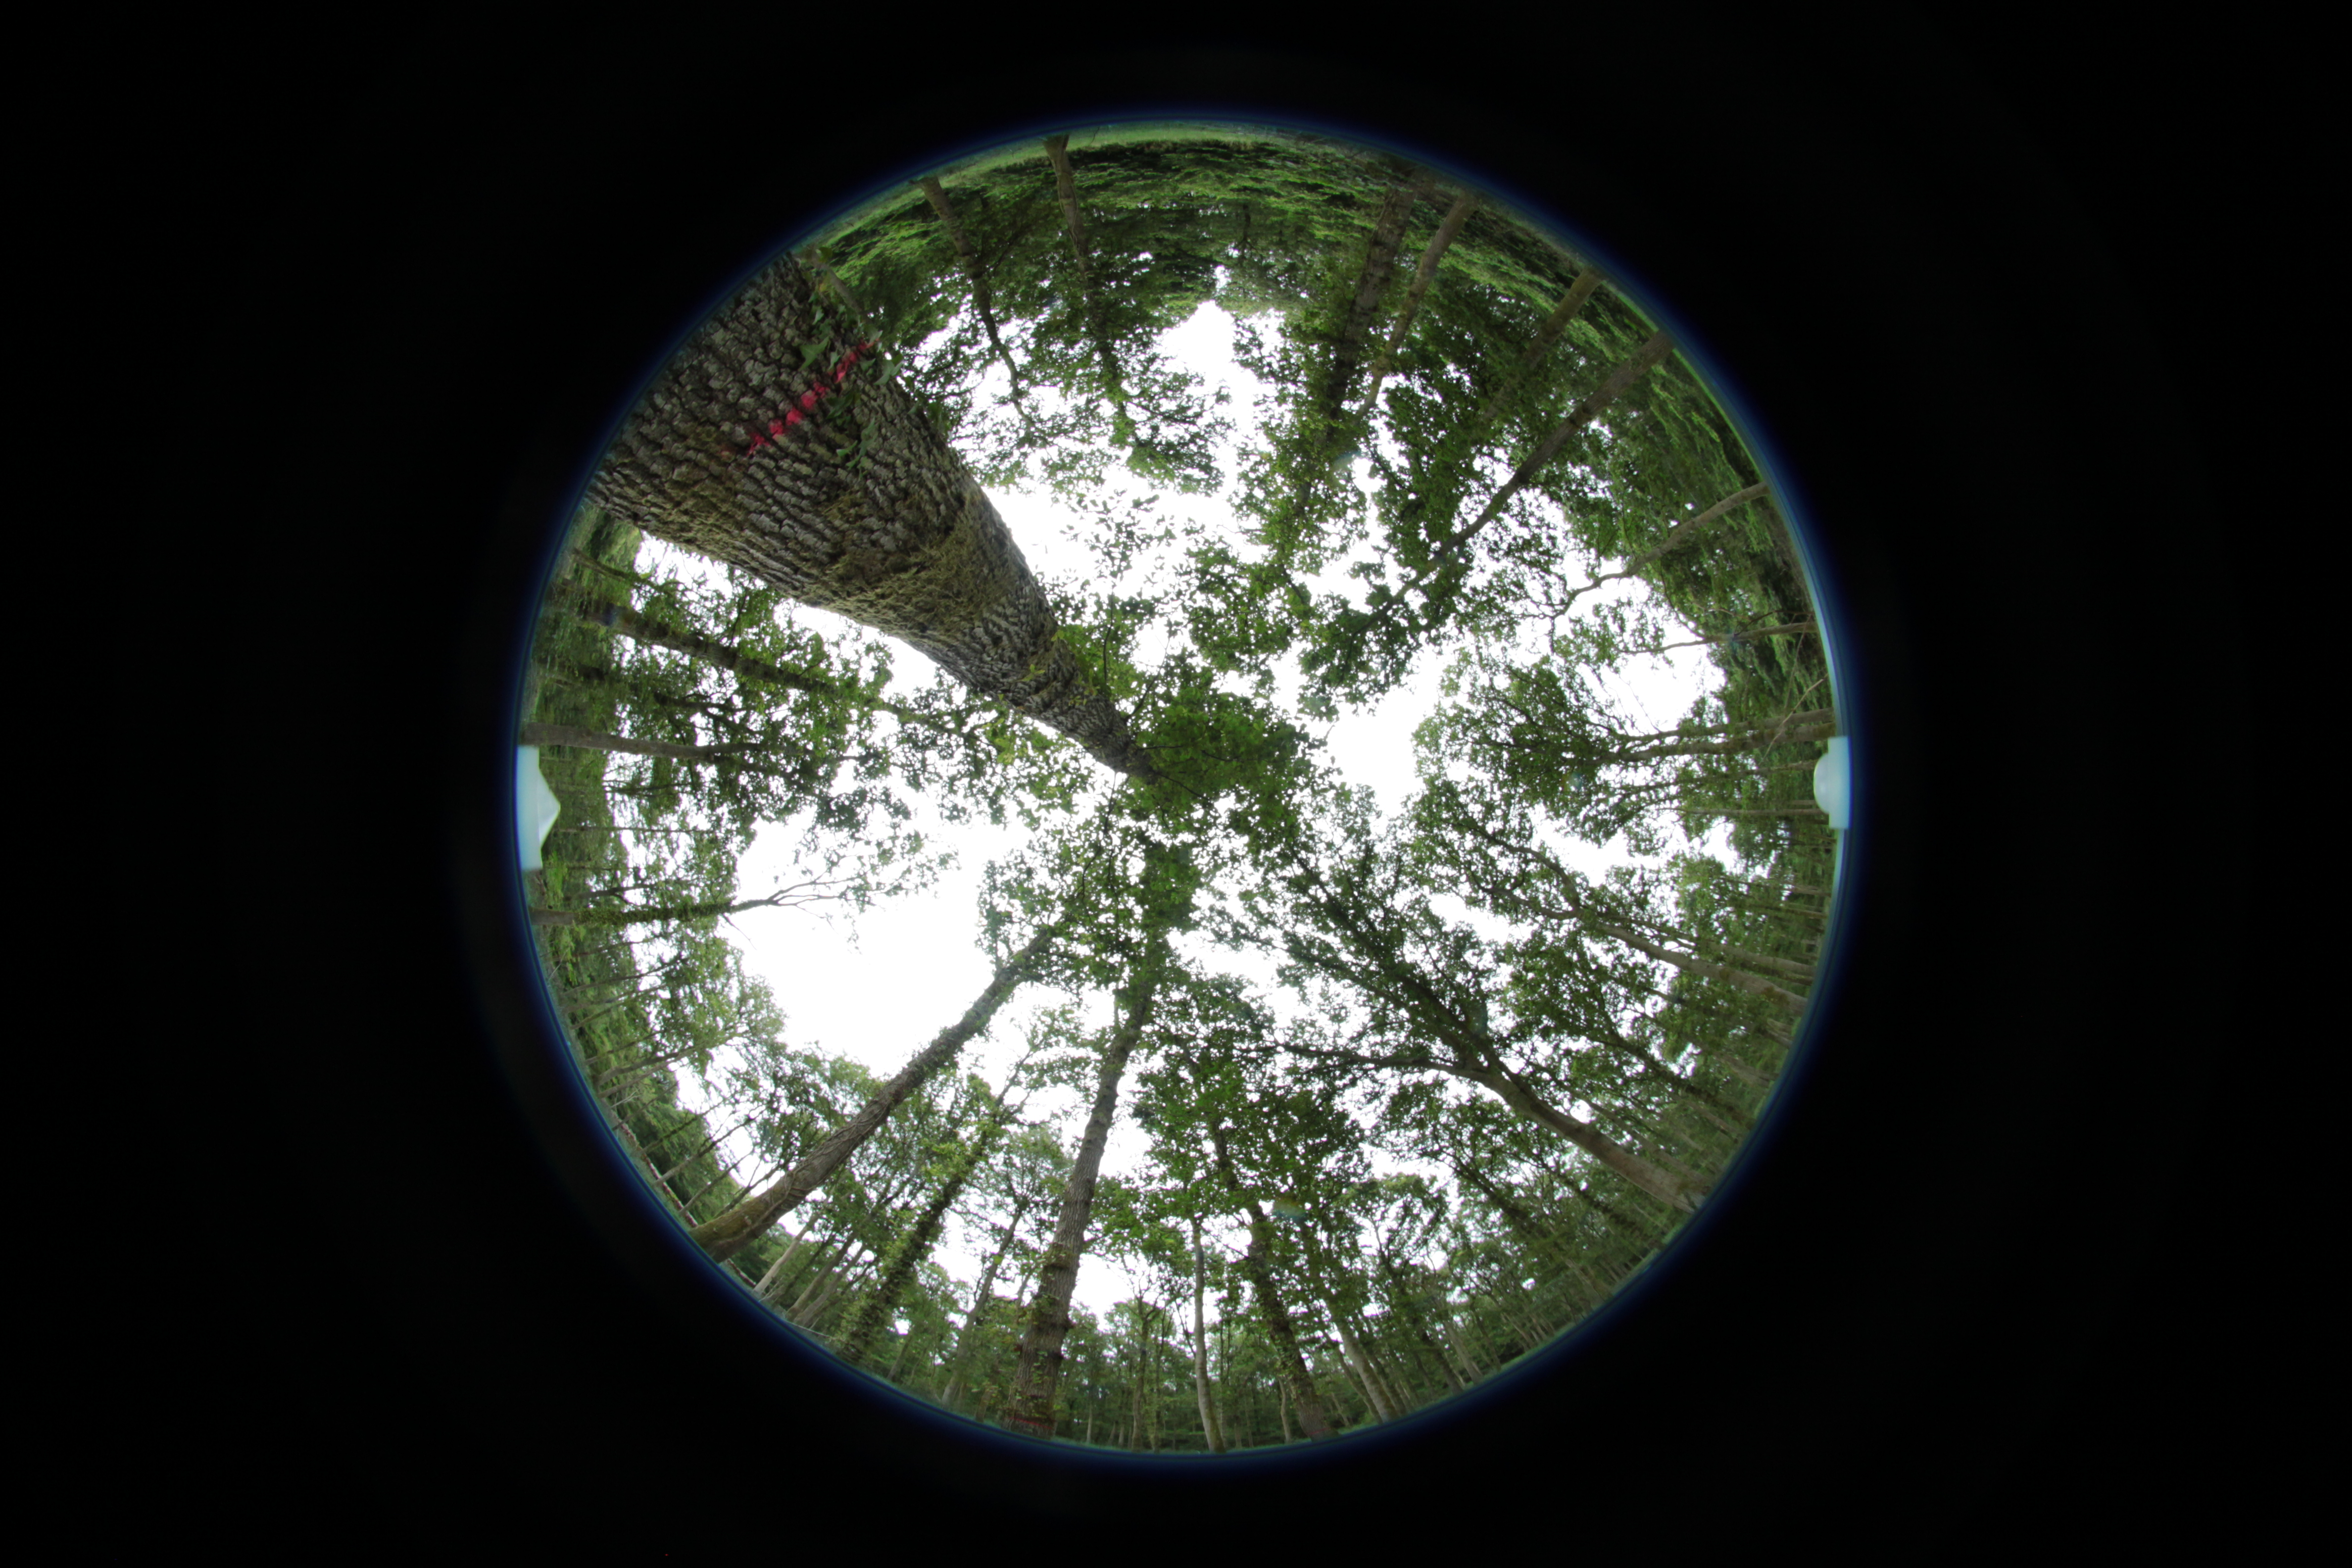
\includegraphics[width=.9\linewidth]{chapter/chapter4/252exp1.jpg}
  \caption{Thinned forest}
  \label{chap4:fig:sub2}
\end{subfigure}
\caption{Hemispherical photographs from the Alice Holt flux site showing the difference between the thinned and unthinned sides of the forest.}
\label{chap4:fig:hemiphotos}
\end{figure}

\subsection{Litter traps}

Finally litter traps were used to find estimates to LAI and leaf mass per area. Here we placed litter traps under the canopy to catch leaf litter as it falls into a bag attached to the bottom of the trap. The bags were changed every week during the litter fall period and the litter sorted into species. Every week the litter was dried in an oven at $70^{\text{o}}\text{C}$ and weighed. This gave us the dry-weight of the leaf litter for the 2015 season. Towards the end of the season we scanned a subsample for each species of 100 leaves to find an area, we then dried and weighed each subsample, a relationship between dry-weight and leaf area was then be built (leaf mass per area) and used to infer the total LAI for each trap once the whole seasons litter has been collected. This method of LAI calculation is the most time consuming.  

A total of six litter traps were established at points along the transects (positions shown in Figure~\ref{chap4:fig:lit_traps}) allowing for comparison with the other methods. The 6 litter traps are not enough to describe the LAI for the research site \citep{kimmins1973some}. We use these litter traps as a point of comparison and validation for the ceptometer and hemispherical photograph estimates of LAI made at the same locations and also for estimates to leaf mass per area. From our litter trap observations we find a leaf mass per area of 29~g~C~m\(^{-2}\) free soluble carbohydrates for both sides of the forest.

\begin{figure}[ht]
    \centering
    \includegraphics[width=0.8\textwidth]{chapter/chapter4/litter_trap.pdf}
    \caption{Litter trap locations for Alice Holt.} \label{chap4:fig:lit_traps}
\end{figure}


\subsection{Comparison of methods} \label{chap4:sec:lai_comp}

In Figure~\ref{chap4:fig:lai_comp07} and \ref{chap4:fig:lai_comp14} we show a comparison of the different methods of estimating LAI for the unthinned and thinned forest respectively. We can see that in all cases LAI derived from the litter traps is always greater than LAI estimated from optical methods, this is expected from previous comparisons \citep{breda2003ground}.
 
Although the ceptometer is the fastest method for measuring LAI it is also the most variable, being extremely sensitive to the solar zenith angle and clear sky conditions. If the sun is low in the sky the radiation will pass through much more photosynthetically active material than if the sun is directly above head, causing spikes in the LAI value. We can see that the LAI estimates from the hemispherical photographs are much less variable than the ceptometer. As discussed in section~\ref{chap4:sec:hemi_photos} the hemispherical estimate is actually of plant area index, as we have not removed trunks and branches from the gap fraction calculation. However, this does not appear to have a great impact on results as hemispherical photograph derived LAI is still the lowest estimate of all three. 

\begin{figure}[ht]
    \centering
    \includegraphics[width=0.8\textwidth]{chapter/chapter4/thinned07.pdf}
    \caption{LAI comparison for unthinned forest. Dots and solid line represent observations made at different points along transects, dotted lines represent the mean of the observations.} \label{chap4:fig:lai_comp07}
\end{figure}

\begin{figure}[ht]
    \centering
    \includegraphics[width=0.8\textwidth]{chapter/chapter4/thinned14.pdf}
    \caption{LAI comparison for thinned forest. Dots and solid line represent observations made at different points along transects, dotted lines represent the mean of the observations.} \label{chap4:fig:lai_comp14}
\end{figure}

\section{Point-centred quater observations}

We used the method of Point-Centred Quarters (PCQ) \citep{dahdouh2006empirical} to determine an estimate of the woody biomass for both unthinned and thinned forest in the Straits Inclosure. The PCQ method is conducted at each sampling point as follows:
\begin{itemize}
\item Using a compass, map 4 regions from the central sampling point
\item Measure the distance from the central sampling point to the nearest tree in each quarter
\item Measure the Diameter at Breast Height (DBH) for each tree (shown in Figure~\ref{chap4:fig:dbh_me}) and record the species 
\end{itemize}
There were 114 points samples along the three transects, from these measurements we derived estimates to tree density and mean DBH for both thinned and unthinned sides of the forest. We then used allometric relationships between DBH and total above ground biomass and coarse root biomass, found in work carried out by Forest Research and in \citet{mckay2003woodfuel}. These relationships were as follows,
\begin{equation}
\text{above ground dry-mass} = 0.0678\times \overline{\text{DBH}}^{2.619}
\end{equation}
and
\begin{equation}
\text{below ground coarse root dry-mass} = 0.149\times \overline{\text{DBH}}^{2.12}.
\end{equation}

This gave us an estimate to the dry-mass in kilograms for the average tree in our sampling area. Assuming that half of all dry-mass is carbon we can find an estimate of total woody and coarse root carbon in g~C~m\(^{-2}\) using the equation,
\begin{multline}
\text{total woody and coarse root carbon} =  \\1000\times0.5\times(\text{above ground dry-mass} + \text{below ground coarse root dry-mass})\times \text{tree density}.
\end{multline}

Forest Research have carried out their own mensuration studies at the site, these have been conducted at the mensuration points shown in Figure~\ref{chap4:fig:transects}. As these plots are included in our transects this means that hopefully our measurements will be comparable with those from Forest Research.  

\begin{figure}[ht]
    \centering
    \includegraphics[width=0.8\textwidth]{chapter/chapter4/dbh_me.pdf}
    \caption{Taking diameter at breast height measurements at Alice Holt.} \label{chap4:fig:dbh_me}
\end{figure}

\section{Flux tower observations and data processing}

Forest Research provided half-hourly raw flux tower data for the Straits Inclosure from January 1999 to December 2015. These consist of the NEE fluxes and meteorological driving data of temperature, irradiance and atmospheric CO\(_{2}\) concentration for use in the DALEC model. The view from the top of the flux tower in the Straits Inclosure can be seen in Figure~\ref{chap4:fig:flux_me}. Forest Research provided this data in the form of multiple excel spreadsheets corresponding to the flux tower measurement record for each year. To prepare this data for use with data assimilation we first had to convert these 16 excel files to one Python readable data file (here we chose NetCDF), this was the further processed. To process the NEE data we first performed \(u^*\) filtering, where any half-hourly flux observation corresponding to a friction velocity of \(0.2~\text{m s}^{-1}\) (this value represents the point at which flux measurements become unreliable and was found by Forest Research) or less were removed from the data set. We then subjected the observations of NEE to quality control procedures similar to those described by \citet{papale2006towards}. For each year of the NEE dataset this procedure involved calculating the standard deviation of both the positive and negative half-hourly observations and then removing any values that were \(\pm 3\) standard deviations away from the yearly positive/negative mean. This was also repeated on a month by month basis. Gap-filling procedures were not applied to the half-hourly NEE dataset so that only true observations were considered for assimilation. To match the time-step of the DALEC model we computed daily NEE observations by taking the mean over the 48 measurements made each day, selecting only days where there was no missing data.  
 

\begin{figure}[ht]
    \centering
    \includegraphics[width=0.8\textwidth]{chapter/chapter4/top_of_flux.pdf}
    \caption{At the top of the Alice Holt flux tower.} \label{chap4:fig:flux_me}
\end{figure}



\chapter{Information content in observations relevant to forest carbon balance}
\label{chap:info_con}
\input{chapter/chapter5/chapter5}

\chapter{Investigating the role of prior and observation error correlations}
\label{chap:error_corrs}
\input{chapter/chapter6/chapter6}

\chapter{Using data assimilation to understand the effect of disturbance on the carbon dynamics of the Alice Holt forest}
\label{chap:disturbance}
%Chapter 6

Insert Chapter here


%more chapters...

\chapter{Conclusion}
\label{chap:conclusion}
%Chapter 1

chapter 8 goes here


It was clear from the first results chapter that in order to better understand the information content in observatnios it is important to improve estimates and representations of uncertainty for both prior modelled estimates and observations.

In the next chapter this is what we did...

\newpage
\addcontentsline{toc}{chapter}{Bibliography}
\def\rightmark{Bibliography}
\def\leftmark{Bibliography}
\renewcommand*{\bibname}{\centerline{\Huge{\bfseries{\scshape{Bibliography}}}}}
\bibliography{../PhD}
%\bibliography{chapter/chapter2/chapter2refs,chapter/chapter3/chapter3refs,chapter/chapter4/chapter4refs,chapter/chapter5/chapter5refs}
\bibliographystyle{./ametsoc}

\end{document}
